\section{Costo previsto del sistema}
Sebbene lo scopo di questa tesi sia evidenziare
l'effetto delle scelte implementative sulla scalabilità del sistema,
l'aspetto economico non può essere ignorato durante la realizzazione di un progetto.
Si cerca quindi di prevedere la spesa effettiva delle risorse utilizzate in base a un utilizzo possibile,
soffermandosi maggiormente sulla dinamica di definizione dei parametri richiesti 
rispetto all'effettiva necessità, 
che può variare in base al mercato dell'applicazione o alla sua maturità.\\
\\
Essendo l'applicazione in fase prototipale, 
si può solamente provare a dedurre l'effettivo utilizzo delle risorse proporzionalmente al carico previsto.
Per il calcolo del costo del sistema si è deciso di considerare un carico 
di cinquemila utenti attivi giornalmente, 
che indica un utilizzo consistente e maturo dell'applicazione.\\
\\
Per stimare il costo del sistema viene usato uno strumento offerto da Azure chiamato Pricing Simulator.
Questo strumento, accessibile online, 
permette di calcolare il costo dell'utilizzo delle risorse in base all'utilizzo che si prevede di farne.
Per ogni servizio, in base alle sue peculiarità, 
viene chiesto l'inserimento di dati specifici per il suo utilizzo.
Per alcuni servizi, in cui era stato adottato il piano di utilizzo più economico, 
è stato necessario assumere l'adozione di un piano 
che permetta effettivamente di gestire il carico previsto.
I costi vengono calcolati mensilmente.\\
\\
Azure Static Web App prevede due tipologie di piani, gratuito o standard.
Il piano gratuito fornisce 100 gigabyte di bandwidth e 
un massimo di 0,5 gigabyte di memoria.
La dimensione attuale dell'applicazione risulta di circa 20 megabyte,
che viene però compressa dal sistema.
Il limite della memoria non risulta quindi un problema,
ma bisogna verificare che non si superi la quantità fornita di bandwidth.\\
\\
La dimensione dei dati ricevuti dal browser in fase di caricamento del sito 
ammonta a un massimo di 10 megabyte.
Questa quantità si riduce notevolmente se il sito è già stato caricato in cache, 
a un massimo stimato di 250 kilobyte.
Considerando che il metodo di fruizione principale del progetto avvenga tramite applicazione,
si stimano 2500 utenti mensili da browser.
Stimando un utilizzo quotidiano dell'applicazione, 
il primo giorno sarà necessario scaricare l'intero sito, 
mentre le volte successive solo aggiornare la cache, 
che porta il calcolo della quantità di dati effettivamente trasferita al seguente:\\
2500 x (10 Mb + 250 Kb x 29) = 43 Gb.\\
I quarantatrè gigabyte così previsti rientrano ampiamente nei cento offerti,
permettendo l'utilizzo del piano gratuito.\\
\\
Per stimare il costo delle Azure Functions è necessario calcolare
le interazioni totali mensili con gli utenti.
Queste vengono previste per 200 richieste giornaliere,
che includono sia richieste in scrittura che in lettura.
Si calcolano così un milione di invocazioni giornaliere, 
per un totale di trenta milioni di chiamate mensili.\\
\\
Dai test si evince una durata media delle funzioni che si aggira sui 200 millisecondi.
Per stare sul sicuro, la durata prevista per richiesta 
viene arrotondata a 250 millisecondi.
Allo stesso modo, si prevede un utilizzo medio di 0.5 gigabyte di memoria per ogni invocazione.
Nel calcolo bisogna considerare le risorse gratuite e
un costo di € 0,000015 per GB/s e € 0,117 per milione di richieste,
portando la spesa totale prevista attorno ai € 60.\\
\begin{figure}[htbp]
    \begin{center}
        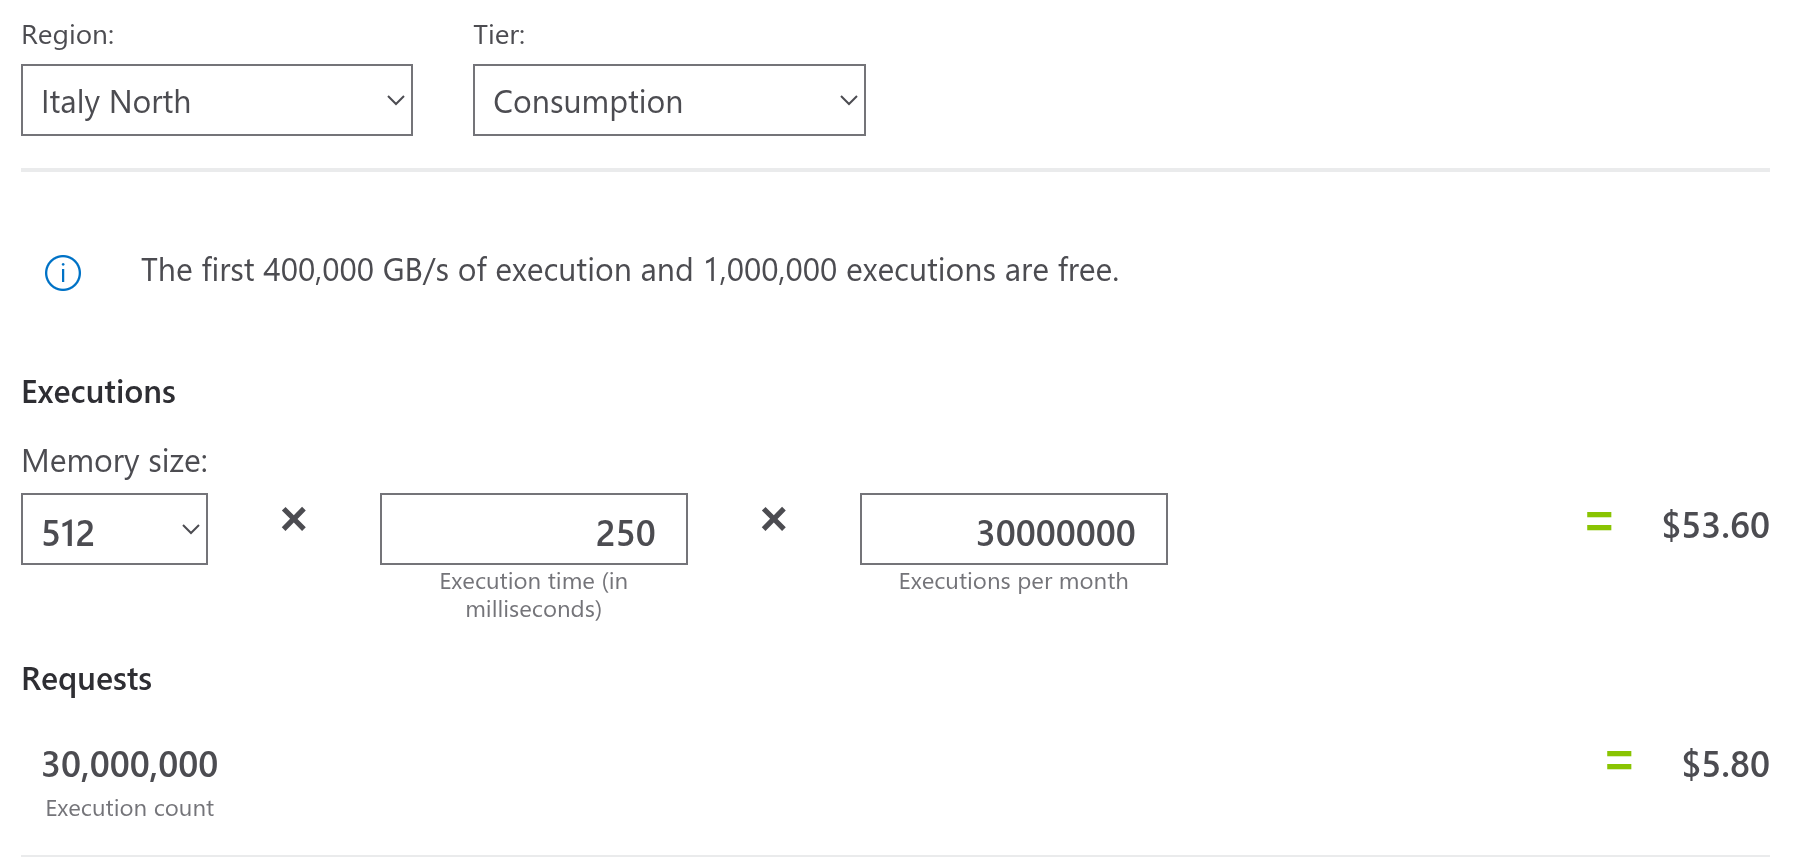
\includegraphics[width=\textwidth]{pricing_functions.png}
        \caption{Calcolo per il costo delle Azure Functions}
    \end{center}
\end{figure}
\\
Il costo del database, implementato con Azure Cosmos DB, 
varia in base alle Request Units al secondo(RU/s) usate.
Ogni richiesta consuma una certa quantità di RU, 
in base al carico computazionale necessario.
Bisogna quindi stimare le richieste al secondo,
e il loro consumo di Request Unit.
Considerando che la quasi totalità delle richieste 
verso le Azure Functions implicano un accesso al database,
le invocazioni per secondo possono essere calcolate 
dividendo le richieste giornaliere per i secondi di una giornata,
facendo così risultare una media di 12 richieste al secondo.\\
\begin{figure}[htbp]
    \begin{center}
        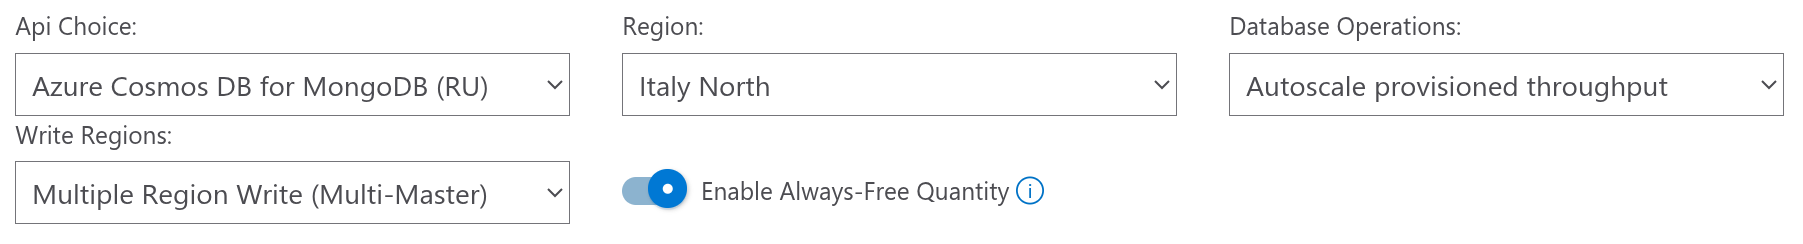
\includegraphics[width=\textwidth]{pricing_settings_cosmos.png}
        \caption{Impostazioni del server Cosmos}
    \end{center}
\end{figure}
\\
Il consumo medio di RU registrato durante i test 
varia tra i 10 e i 20 RU per richiesta.
Per sicurezza, si considera il consumo medio di un'operazione sul database
di 30 RU.
Risulta così una media di 360 RU/s,
che non fornisce però informazioni sul picco del carico. 
Utilizzando un piano di tipologia autoscale,
che modifica in automatico le risorse del database in base al carico effettivo,
bisogna stabilire il carico massimo che si prevede il database debba sostenere,
tenendo però presente che la quantità minima di risorse sempre stanziate sarà del suo 10\%.\\
\\
Non essendo in possesso di dati relativi all'effettivo utilizzo dell'applicazione,
Stimiamo un utilizzo massimo pari a 5 volte quello previsto, 
pari a 60 richieste al secondo.
Questo porta a un massimo di 1800 RU/s, con una media prevista del 20\%.
Sottraendo i primi 1000 RU/s e moltiplicando i restanti per il costo orario di € 0,014, 
il costo totale previsto per l'utilizzo di Azure Cosmos si aggira intorno ai € 17.\\
\begin{figure}[htbp]
    \begin{center}
        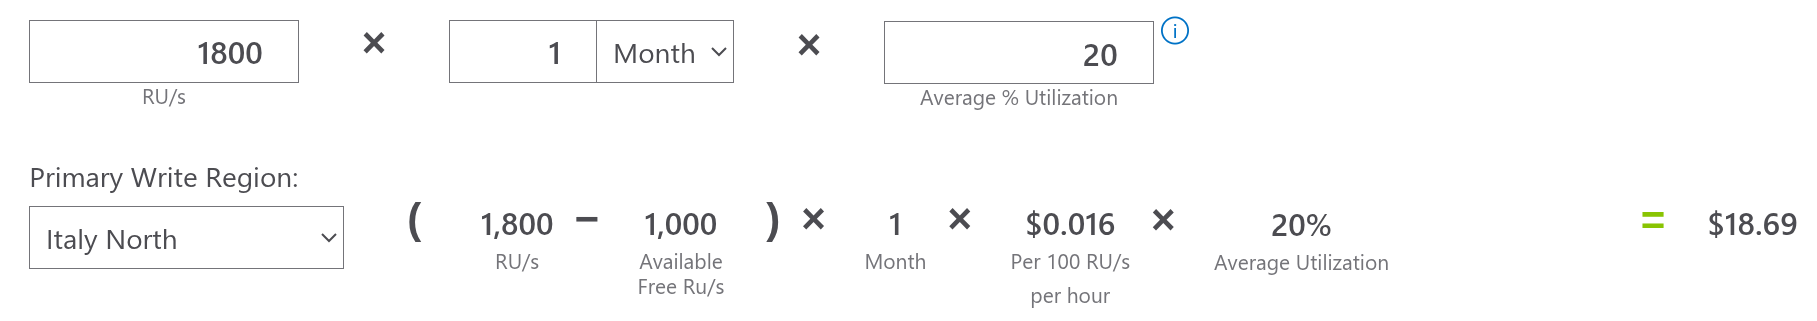
\includegraphics[width=\textwidth]{pricing_cosmos.png}
        \caption{Calcolo per il costo di Cosmos}
    \end{center}
\end{figure}
\clearpage
Per poter garantire la gestione totale dell'esecuzione dei messaggi
è necessario impostare il piano Standard di Service Bus.
Prevede un costo di base orario di € 0,012, 
più € 0,71 per ogni milione di messaggi, 
includendo però nel prezzo i primi 13 milioni.
Stimando le operazioni in scrittura
(che sono quelle che richiedono la propagazione)
a un terzo di quelle totali, si prevedono 9 milioni di messaggi mensili,
riducendo la spessa al solo costo della macchina, che ammonta così a circa € 9.\\
\\
Le operazioni di aggiornamento sono le stesse che richiedono 
l'invio delle notifiche, scatenate tramite messaggio inviato su una Azure Storage Queue.
Ogni richiesta comporta una scrittura sulla coda,
che verrà presa in carico da una funzione, con un'operazione di lettura.
Questo comporta 9 milioni di operazioni in lettura e altrettante in scrittura.
A un costo di € 0,0035 ogni 10.000 operazioni, comporta una spesa di € 6,40, 
a cui si aggiunge € 1 per la capacità della coda che, per sicurezza, è stata stimata a 25 gigabyte.
Questa quota difficilmente viene raggiunta in quanto un messaggio, 
dopo essere stato letto, dovrebbe essere eliminato.\\
\begin{figure}[htbp]
    \begin{center}
        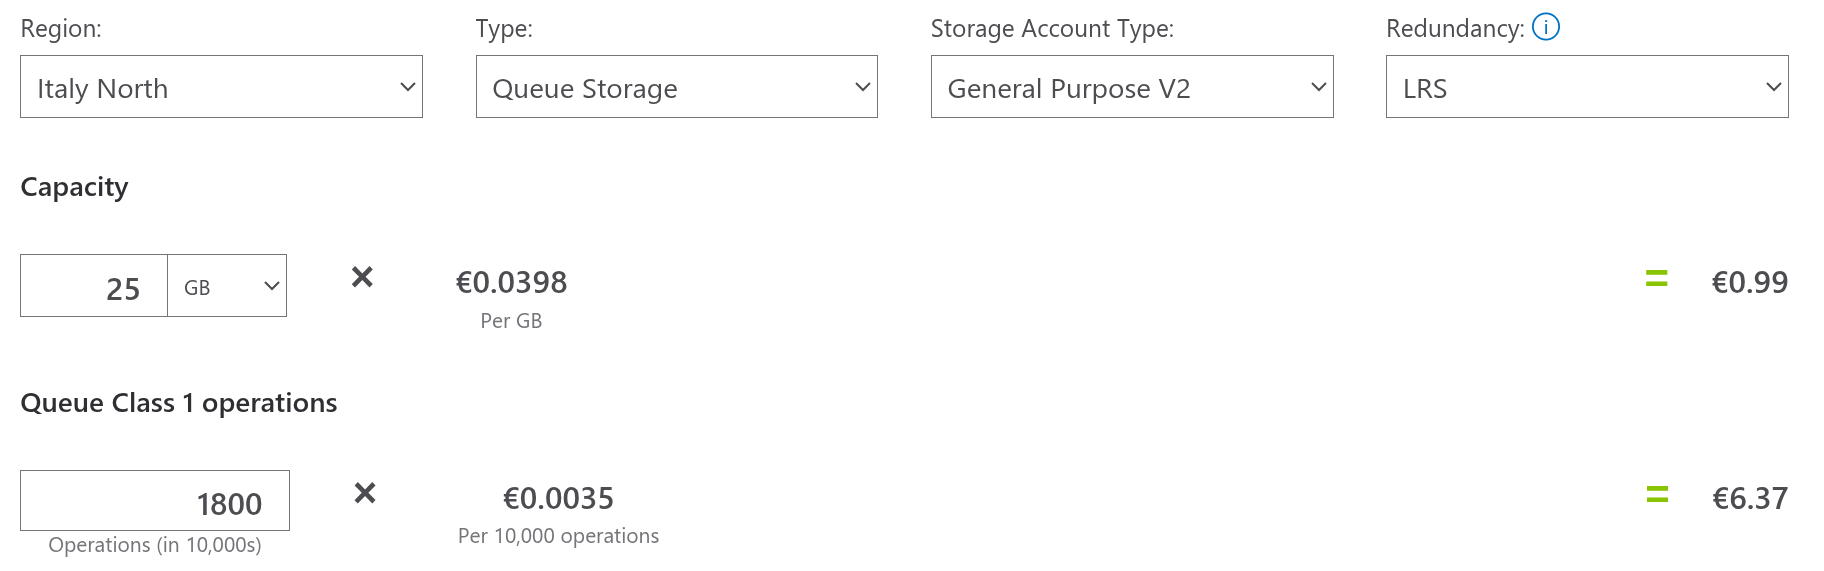
\includegraphics[width=\textwidth]{pricing_queue.png}
        \caption{Calcolo per il costo di Azure Storage Queue}
    \end{center}
\end{figure}
\\
Per l'invio delle notifiche si utilizza Azure PubSub.
La versione gratuita non è più sufficiente, 
potendo garantire un massimo di 20 connessioni contemporanee.
Si stima però che, modificando il contratto a Standard, una istanza sia sufficiente,
la quale, con un costo orario di € 0,0594, ammonta da sola a € 44 mensili.
Stimando la dimensione media dei messaggi delle notifiche a 1 Kb,
e prevedendo una media di 10 utenti attivi per ogni notifica, 
la dimensione totale dei messaggi così inviati con PubSub 
dovrebbe ammontare attorno a 9.000.000 x 1 Kb x 10 = 90 Gb.
Il costo per l'invio dei messaggi risultà così pari a € 13, per un totale di circa € 56 mensili.\\
\\
Per il calcolo del costo di Azure Blob Storage, 
che viene usato per salvare le immagini,
viene stimato un carico di un'immagine al giorno per utente,
o di 30 immagini al mese.
Azure Blob Storage prevede un costo in base alla dimensione totale dei dati salvati,
a cui si aggiunge il costo computazionale necessario per aggiungere o trovare le immagini.
Considerata una dimensione media per immagine (compressa) di 200 Kb,
ogni mese vengono aggiunti 30 x 5000 x 200 Kb = 30 Gb.
Dopo un anno di utilizzo stimiamo quindi una dimensione totale di 360 Gb, 
per una spesa mensile di € 6.\\
\\
Si stima inoltre che un utente guardi giornalmente 3 eventi nel dettaglio, 
i quali sono mediamente condividi con 10 utenti.
Considerando il carico di una immagine al giorno per utente,
ogni utente esegue, al giorno, 3 richieste di elenco e 30 di lettura.
Si calcolano così 150.000 richieste di scrittura,
450.000 richieste di elenco,
e 4.500.000 richieste di lettura.
Con un prezzo di € 0,047 ogni 10.000 invocazioni per i primi due casi,
e di € 0,004 ogni 10.000 invocazioni per le letture,
il costo computazione ammonta a € 4,50.
La spesa totale per il servizio viene quindi stimata a € 10,5.\\
\\
Per il Key Vault bisogna stimare la frequenza 
con cui le Functions necessitano di recuperare i segreti per accedere agli altri servizi.
Si stima che, come minimo, ogni richiesta abbia bisogno di almeno un segreto,
ad esempio per accedere al database.
Le Azure Functions sono però strutturate per riutilizzare 
l'ambiente di esecuzione, se le risorse computazionali lo permettono.
Questo consente di riutilizzare i segreti recuperati dalle funzioni invocate precedentemente.
Si stima quindi che il Key Vault venga interrogato una volta ogni dieci richieste,
per un totale di 3 milioni al mese.
Per un costo di € 0,027 ogni 10.000 invocazioni,
la spesa totale di Azure Key Vault viene prevista per circa € 8.\\
\\
L'ultima risorsa utilizzata all'interno dell'ecosistema Azure è Virtual Network, 
il cui utilizzo è però gratuito.
Infine, il servizio per l'autenticazione, Firebase Authentication,
risulta anch'esso gratuito, non superando la soglia dei 50.0000 utenti attivi mensili.
\clearpage
\begin{figure}[htbp]
    \begin{center}
        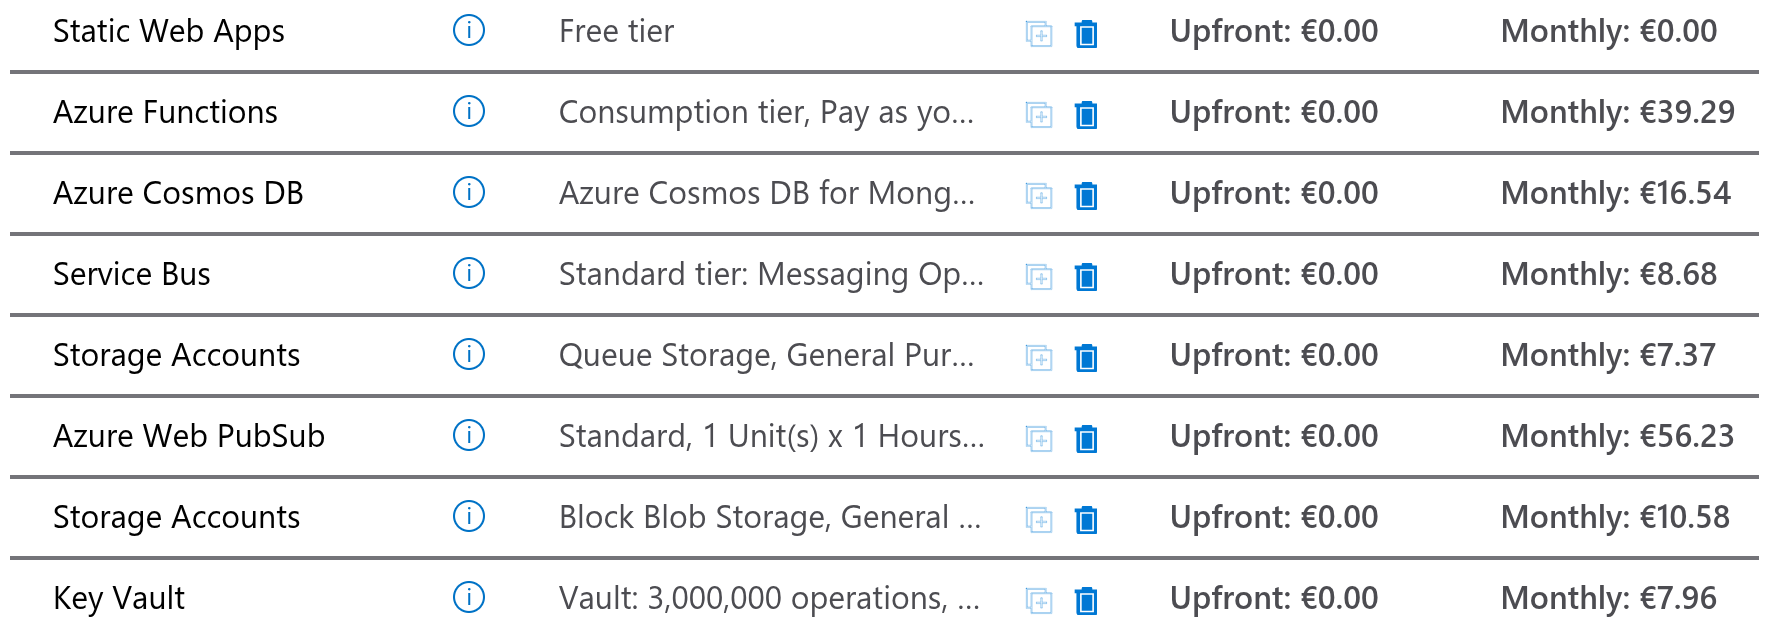
\includegraphics[width=\textwidth]{pricing_general.png}
        \caption{Riassunto dei costi previsti delle risorse Azure}
    \end{center}
\end{figure}
Il costo totale previsto per fornire il servizio a 5000 utenti ammonta quindi a circa € 150.
Viste tutte le stime assunte sull'utilizzo del sistema 
questa cifra è da considerarsi indicativa.
Fornisce però una dimensione iniziale sul costo da prevedere per l'esecuzione del sistema.
Come appena presentato, il prezzo può infatti essere correlato al numero di utenti attivi, 
tenendo però presente la scalabilità specifica di ogni servizio.\\
\\
L'analisi di questo calcolo evidenzia quanto sia significativo
l'impatto di Azure PubSub sul totale. 
Visto il ruolo nel sistema, 
il suo utilizzo risulta sicuramente degno di revisione,
per trovare soluzioni alternative che possano fornire 
un servizio di pari qualità, a un prezzo minore.


\clearpage
\chapter*{Conclusione}
\addcontentsline{toc}{chapter}{Conclusione}
L'obiettivo di questa tesi era mostrare a che livello e in che misura
il requisito della scalabilità e l'utilizzo delle risorse in cloud impattano sulla realizzazione di un'applicazione.\\
\\
Durante la fase di analisi è stato evidenziato quali fossero i punti critici del progetto.
Si sono quindi affiancate a ogni componente scelto le necessità a cui dovevano rispondere,
eventualmente approfondendo le molteplici offerte presenti sul mercato.
La scelta è stata determinata dalle tecnologie e funzionalità che presentavano, 
influenzando in maniera decisiva l'approccio da usare
nella progettazione del codice.
Sono state quindi affiancate le scelte implementative implicate dall'utilizzo dei vari servizi.\\
\begin{figure}[htbp]
    \begin{center}
        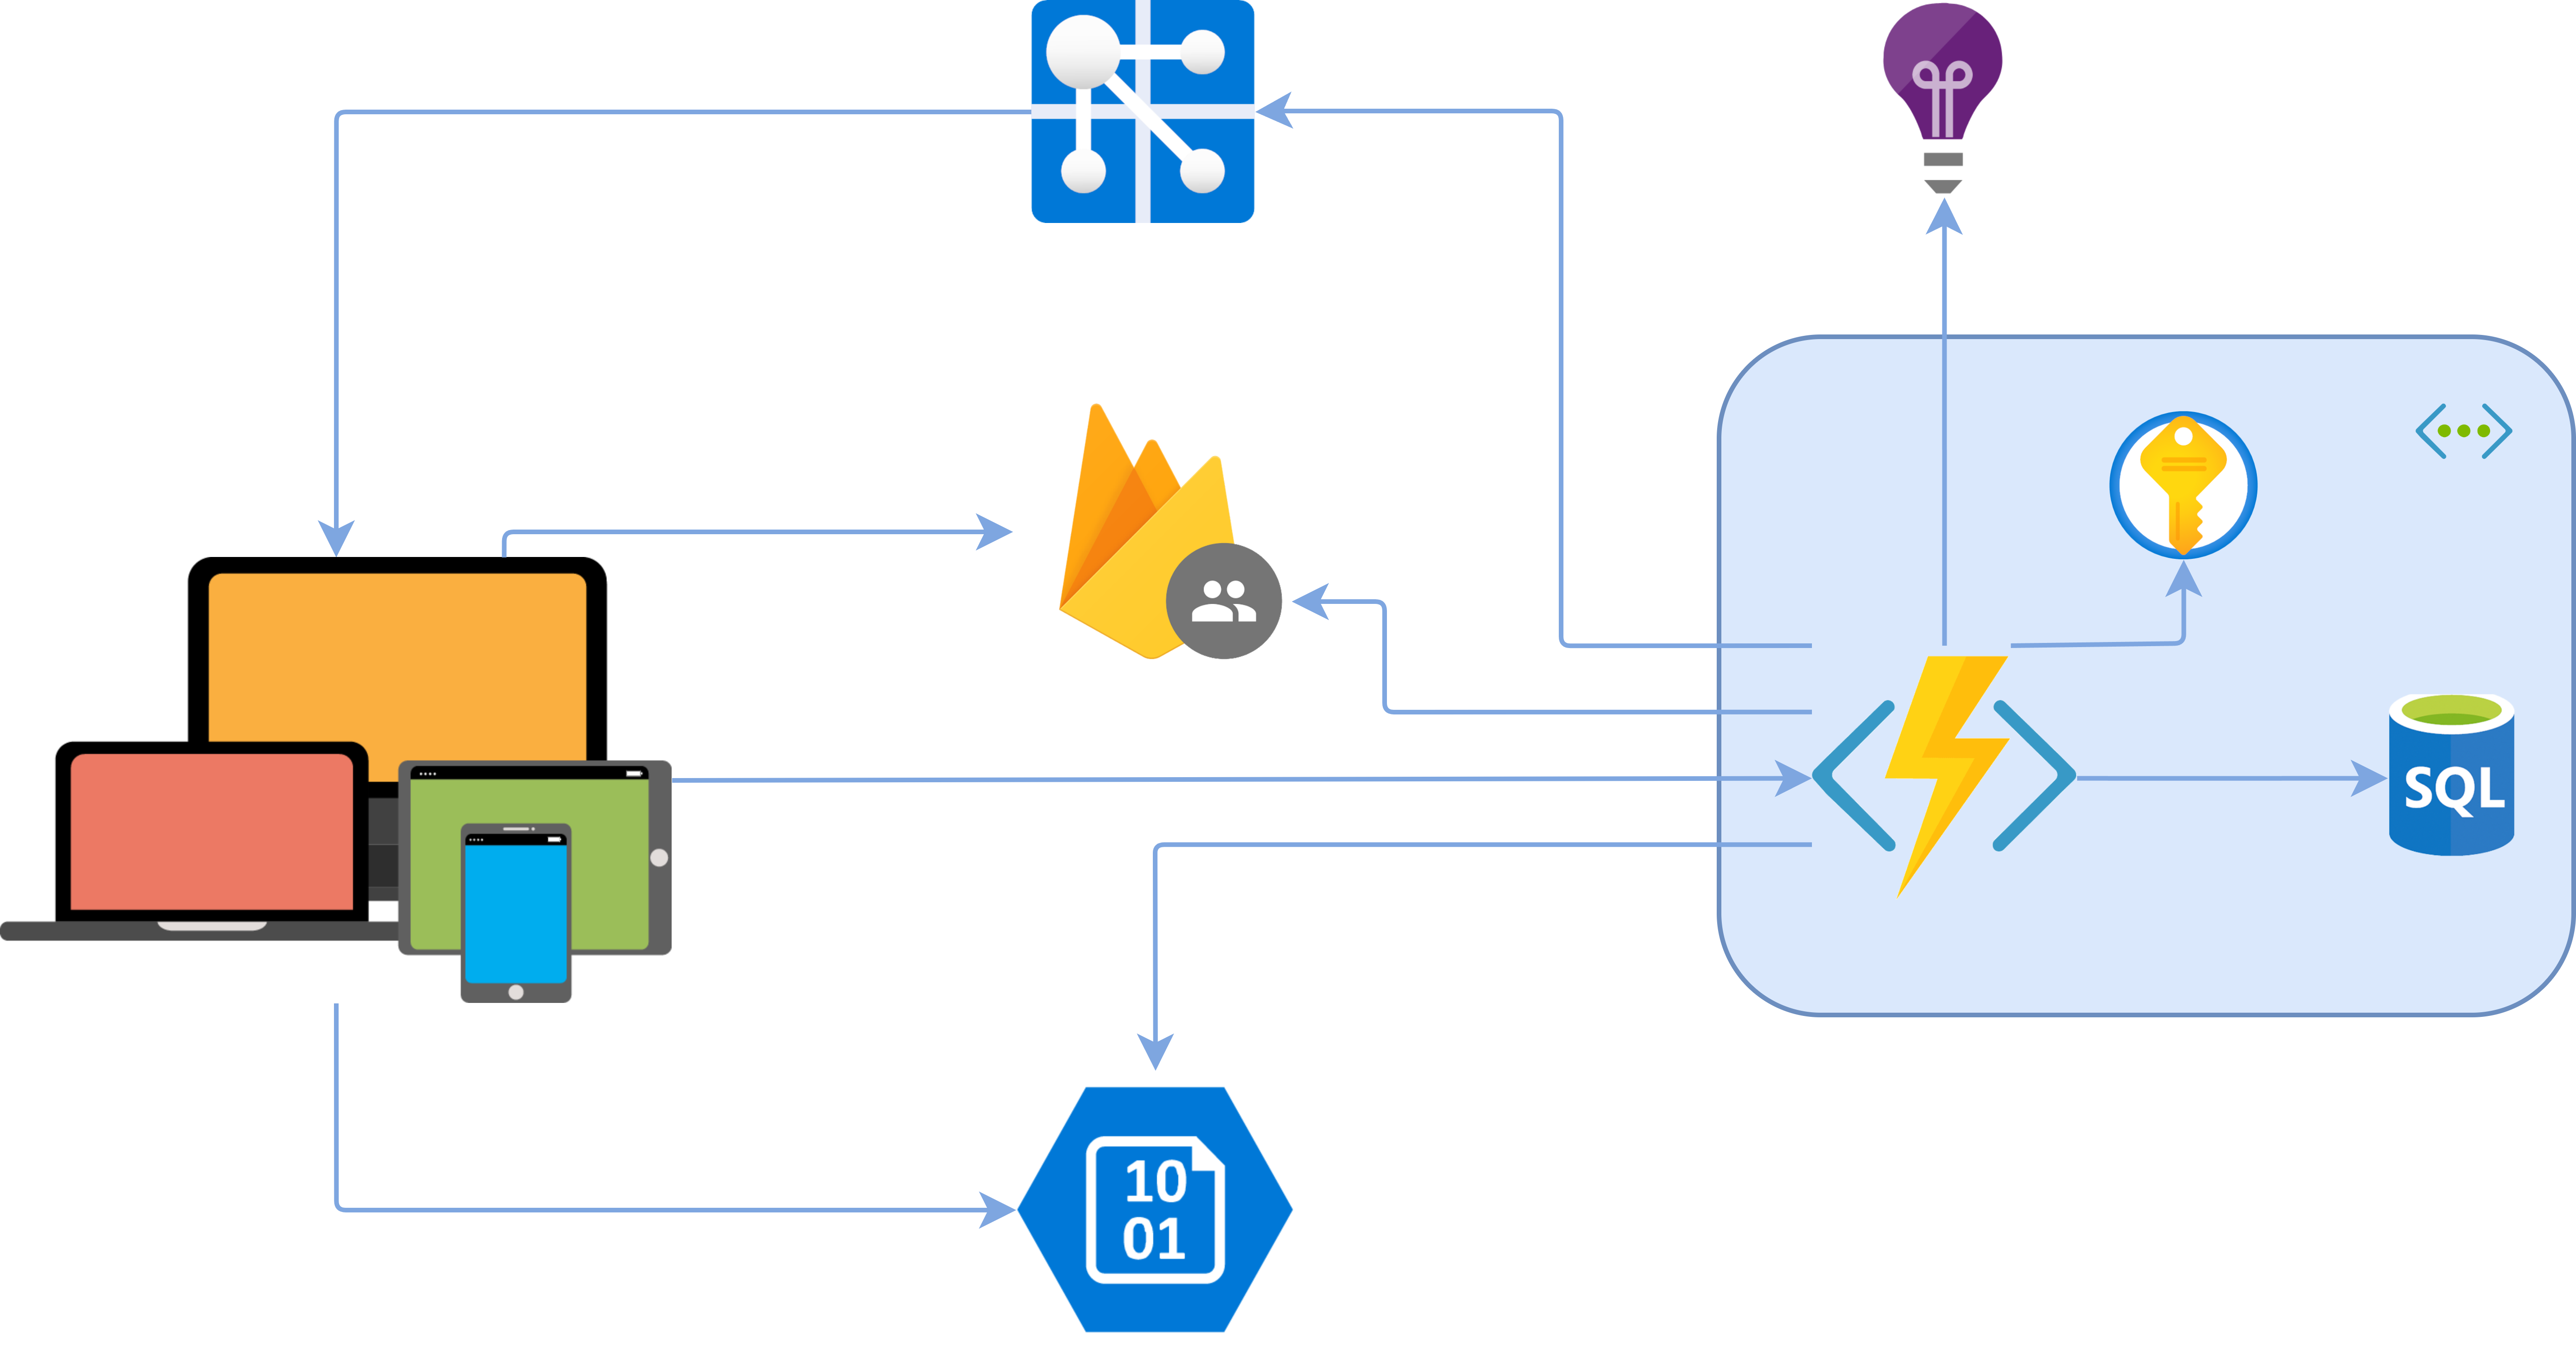
\includegraphics[width=\textwidth]{ImplementazioneArchitettura.png}
        \caption{Grafico dell'architettura di WYD}
    \end{center}
\end{figure}
\clearpage
La fase di realizzazione ha visto lo sviluppo di un client utente intuitivo 
e di un server scalabile ed efficiente, sfruttando la tecnologia serverless.
Una particolare attenzione è stata prestata ai meccanismi di autenticazione, 
alla sicurezza dei dati e al monitoraggio continuo dei servizi.
La gestione della persistenza è stata affrontata 
attraverso l'implementazione di un database non relazionale distribuito,
scelta che ha comportato il principale impatto sulle dinamiche del progetto.
Gli è stato inoltre affiancato lo sviluppo 
di una memoria locale per la cache e la comunicazione in tempo reale, 
elementi cruciali per la reattività dell'applicativo.
Un capitolo significativo è stato dedicato al recupero e al salvataggio dei dati multimediali, 
essenziali per la funzionalità di condivisione in tempo reale di Wyd.\\
\\
L'integrazione tra le tecnologie cloud ha richiesto 
un approccio progettuale orientato alla separazione delle responsabilità, 
alla gestione della consistenza eventuale e alla resilienza in caso di errori o richieste concorrenti. Ciò ha condotto all'adozione di pattern moderni, 
come la denormalizzazione, i trigger su modifiche, 
l'uso di code per la propagazione degli eventi e 
notifiche in tempo reale attraverso canali dedicati.\\
\\
I risultati ottenuti durante i test di carico hanno confermato 
la qualità delle scelte architetturali adottate: 
il sistema dimostra di sostenere centinaia di richieste al secondo 
senza degrado percettibile delle prestazioni, 
mantenendo al tempo stesso un basso tempo di latenza.\\
\\
In definitiva, il percorso intrapreso ha mostrato 
come la realizzazione di un'applicazione distribuita e scalabile 
non sia il frutto di un processo lineare, 
ma di un dialogo costante tra le esigenze funzionali, 
i vincoli tecnologici e le opportunità offerte dai servizi cloud-native. 
Ogni tecnologia adottata ha influito sulle logiche implementative, 
imponendo precise scelte progettuali, 
sia in termini di prestazioni che di costi.\\
\\
L'auspicio è che le considerazioni sviluppate 
possano offrire un contributo utile non solo alla valutazione di Wyd come progetto,
ma anche come punto di partenza per l'approfondimento dei principi e delle pratiche 
legate allo sviluppo di applicazioni moderne, condivise e scalabili.
\clearpage

\section{Sviluppi futuri}

Wyd può essere ampliata nelle sue funzionalità,
con conseguenze sull'infrastruttura che possono essere nulle o molto impattanti.\\
\\
L'architettura attuale guadagnerebbe sicuramente in prestazioni dall'introduzione
di una cache tra le Azure Functions e il database.
È inoltre bene rivedere l'utilizzo delle websocket per le informazioni in tempo reale, 
considerato l'impatto previsto di Azure PubSub sui costi totali.\\
\\
L'implementazione di eventi pubblici è sicuramente il principale passo logico successivo 
per rendere Wyd un'applicazione di ampio utilizzo.
Questo comporta la realizzazione di una piattaforma dedicata,
che riceva gli eventi e ne gestisca la condivisione,
tenendo traccia di tutti i rapporti tra profili che seguono e 
profili che possono pubblicare.\\
\\
Con la creazione di eventi pubblici ha senso prevedere un sistema 
per gestire la prenotazione e l'organizzazione degli eventi,
dalle liste di attesa alle vendite dei biglietti.
La necessità di garantire la robustezza del servizio,
introducendo logiche di controllo dei ruoli e di traffico monetario,
comporta requisiti specifici di affidabilità e consistenza 
a cui l'infrastruttura dovrà rispondere.\\
\\
Vista la crescente attenzione alla privacy, 
alla protezione dei dati e alla dipendenza dovuta all'utilizzo di servizi esterni,
si prevede di sviluppare un applicativo gemello 
che possa essere distribuito su un unico server dedicato,
per fornire la possibilità a terzi di eseguire su macchine proprie.
Il programma vedrebbe quindi un'infrastruttura fisica completamente diversa,
ma la sua implementazione continuerebbe a seguire
tutti i principi adottati per mantenere il codice scalabile,
fornendo così un prodotto comunque resistente a carichi differenti, seppure ridotti.
Questo diminuirebbe inoltre il numero di modifiche da introdurre nel codice.\\
\\
Infine, ulteriori sviluppi potranno comprendere, in base alle necessità degli utenti:
\begin{itemize}
    \item La visualizzazione degli impegni degli altri profili
    \item L'implementazione di una chat per ogni gruppo
    \item Strumenti utili all'organizzazione dei gruppi, quali:
          \begin{itemize}
              \item form per combinare le disponibilità reciproche
              \item appunti condivisi(liste della spesa o note su chi porta cosa)
              \item calcolo delle spese compiute da ciascun componente
          \end{itemize}
    \item Una funzionalità di ricerca degli eventi o dei profili pubblici
\end{itemize}
\clearpage